\section{Association Analysis}
\subsection{Introduction (*)}

L'analisi di associazione riporta al concetto di causalità di variabili: dati certi valori di attributi cosa posso dire del valore di un altro attributo?

Le regole associative permettono di prendere delle scelte molto operative in diversi ambiti, in particolare in quello che viene chiamato \textit{market busket analysis}. 
Il problema del carrello tratta il posizionamento di prodotti in un negozio. Si sa che all'acquisto di un certo prodotto si tende a acquistare altri prodotti connessi, quindi si cercano queste associazioni basandosi sul carrello della spesa dei clienti (appunto market basket) per poi capire come impostare la disposizione sugli scaffali.

\textbf{Obiettivo}: identificare quali siano gli \textbf{item associati} per poter prendere delle decisioni. In sostanza si generano \textbf{Regole associative} formate da coppie di insiemi \textit{antecedente} e \textit{conseguente}.

es. \{Beer\} $\rightarrow$ \{swiss cheese\} 

\quad \{antecedente\} $\rightarrow$ \{conseguente\}\\
\textbf{NB}: non \`e una causalit\`a ma un'associazione

L'analisi si basa sullo studio di due diversi dataset:
\begin{itemize}
	\item Product set: contiene informazioni legate ai prodotti come il nome e il prezzo
	\item Transaction set: contiene informazioni legate agli acquisti dei clienti, ogni record corrisponde ai prodotti presenti nel carrello del cliente
\end{itemize}

Si organizza il dataset delle transazioni in formato binario, ovvero ogni colonna indica se in una data transazione un certo prodotto sia o meno presente.

\begin{figure}[H]
	\centering
	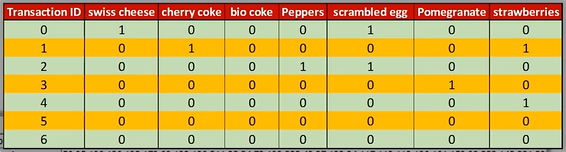
\includegraphics[height=0.25 \linewidth]{association/pict/transaction_set_bin.png}
	\caption{esempio: transaction set binarizzato}
\end{figure}
\clearpage
\noindent
Consideriamo:

$I = \{i_1, i_2,...,i_d\}$ il set di tutti gli item nel market basket

$T = \{t_1,t_2,...,t_N\}$ l'insieme di tutte le transazioni

\begin{defn}
	Una collezione di zero o più item è chiamata \textbf{Itemset}.
\end{defn} 
\begin{defn}
	Se un itemset contiene k item \`e detto \textbf{K-Itemset}.
\end{defn}
\begin{defn}
	L'itemset che non contiene alcun elemento è detto \textbf{empty set}.
\end{defn}
\begin{defn}
	La \textbf{transaction width} è il numero di item presenti in una transazione
\end{defn}
	 
Una transazione $t_j$ contiene l'itemset $X$, se $X$ è un sottoinsieme di $t_j$.

\begin{defn}
	Il \textbf{Support count} è il numero di transazioni che contentono uno specifico itemset.

\[ \sigma(X) = |\{t_i | X \subseteq t_i, t_i \in T\} \]
\end{defn}

\begin{defn}
Una \textbf{regola di associazione} viene rappresentata come:

$X \rightarrow Y$

dove $X$ e $Y$ sono itemset disgiunti ($X \cap Y = \emptyset$).
\end{defn}
Una regola viene valutata in termini di \textit{supporto} e di \textit{confidenza}.

\begin{defn}
	\textbf{Support} determina quanto spesso una regola sia applicabile dato un data set:
	
	\[s\{x \rightarrow Y\} = \frac{\sigma(X \cup Y)}{N}\]
\end{defn}
\begin{defn}
	\textbf{Confidence} determina quanto frequente Y \`e presente in una transazione che contiene X (si assume che l'universo sia rappresentato partendo da X):
	
	\[c\{x \rightarrow Y\} = \frac{\sigma(X \cup Y)}{\sigma(X)}\]
\end{defn}

\textbf{Es}. \\
$X = \{swiss cheese, cheddar\}$, $Y = \{diet coke\}$\\
Assumiamo che:
\begin{itemize}
	\item $\sigma(x) = 8$ (support count)
	\item $N = 20$ (numero di transazioni)
	\item $\sigma(x,y) = 6$ 
\end{itemize}
Allora il support e la confidence della regola $X \rightarrow Y$ sono:

\[s\{X \rightarrow Y\} = \frac{\sigma(X \cup Y)}{N} = \frac{6}{20} = 0.3\]

\[c\{x \rightarrow Y\} = \frac{\sigma(X \cup Y)}{\sigma(X)} = \frac{6}{8} = 0.75\]

Perché utiliziamo il supporto:
\begin{itemize}
	\item se troppo basso potrebbe esserci un'associazione casuale
	\item potrebbe non valere la pena seguire associazioni che si applicano in modo poco significativo dal punto di vista dei profitti 
\end{itemize}
Il concetto di supporto è utilizzato per eliminare regole non desiderate e condivide interessanti proprietà che possono essere sfruttate per la ricerca di regole associative efficaci.

La confidenza \`e molto importante perché misura l'affidabilità dell'inferenza e:
\begin{itemize}
	\item un' alta confidenza significa che Y sarà molto presente in transazioni con X 
	\item si stima la probabilit\`a condizionata di Y dato X
\end{itemize}
\begin{defn}
\textbf{Association Rule Mining Problem} può essere formalmente definito come: dato un set di transazioni T, trovare tutte le regole con $support \ge minsup$ e $confidence \ge minconf$, dove $minsup$ e $minconf$ sono i threshold corrispondenti alle due misure.
\end{defn}

\textit{Approccio a forza bruta} di association rule non è molto praticabile in quanto i tempi di computazione aumentano in modo esponenziale: 

$R = 3^d - 2^{d+1} + 1$.

\begin{figure}[H]
	\centering
	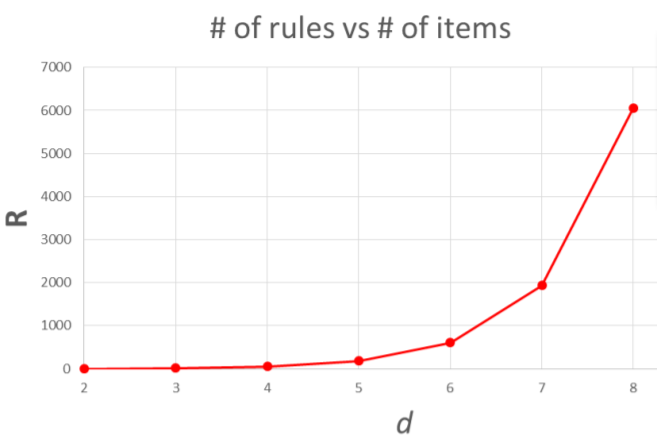
\includegraphics[height=0.4 \linewidth]{association/pict/brute_force.png}
	\caption{numero di regole calcolate in base al numero di itemset}
\end{figure}

Una strategia comunemente adottata in molti algoritmi è quella di decomporre il problema in 2 grandi supertask:
\begin{itemize}
	\item\textit{Generazione dei frequenti itemset}: specifichiamo tutte e sole quelle regole per cui il supporto è maggiore del $minsup$, gli itemset generati sono chiamati \textbf{Frequent Itemset}
	\item \textit{Generazione delle regole}: estriamo tutte le regole con alta confidenza (maggiore di $minconf$) dai Frequent Itemset trovati precedentemente, queste regole vengono chiamate \textbf{Strong Rules}
\end{itemize}
\noindent
La complessità maggiore è richiesta dalla generazione dei Frequent Itemset.


\subsection{Rule Extraction}

Per comprendere l'inefficienza della generazione con l'approccio forza bruta pensiamo a questo esempio:
\begin{figure}[H]
	\hspace{-0.7 cm}
	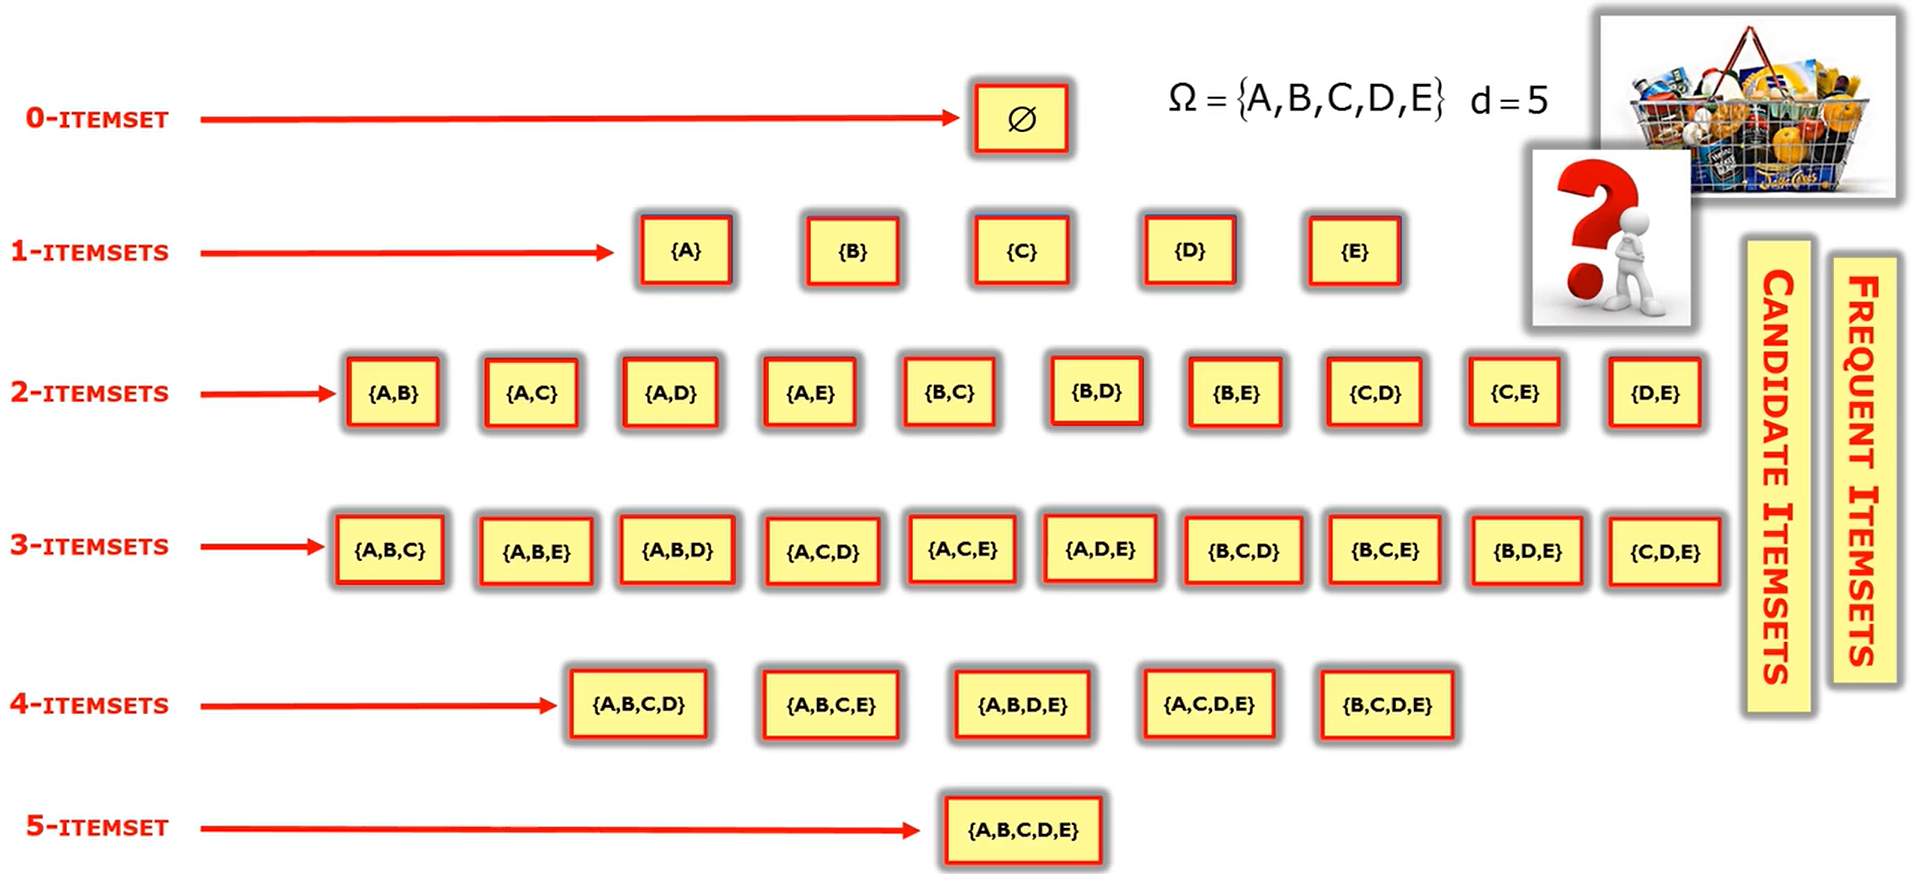
\includegraphics[height=0.5 \linewidth]{association/pict/k-itemset.png}
	\caption{k-itemset brute-force}
\end{figure}
\begin{defn}
	\textbf{Candidate Itemset}: l'insieme di tutti gli itemset che possiamo formare. Avranno un numero di item diverso. 
\end{defn}
Nel nostro caso il numero di itemset candidato è: $M = 2^{d} - 1 = 2^5 -1 = 31$

Come si può notare abbiamo un sistema a doppio cono che è tipica delle distribuzioni binomiali. Una volta che li abbiamo considerati tutti ci interessano solo i più frequenti. \\
Se usassimo la forza bruta dovremmo calcolare per ogni itemset candidato il suo support count, e vedere se il suo supporto lo configura come un itemset frequente (molto dispendioso). 

I confronti da effettuare sono nell'ordine di $O(NMw)$, dove:
\begin{itemize}
	\item $N$ = numero di transazioni
	\item $M$ = numero di itemset candidato
	\item $w$ = massima lunghezza delle transazioni
\end{itemize} 

È decisamente troppo come numero di confronti contando che molti dei quali sono inutili o poco significativi.

Vi sono due approcci per ridurre il costo computazionale della generazione di itemset frequenti:
\begin{itemize}
	\item ridurre il numero di candidati itemset ($M$). Il principio Apriori \`e un metodo per eliminare alcuni candidati itemset senza contare il support count. 
	\item riduce il numero di confronti anzich\`e controllare tutte le possibili combinazioni, lo si fa con strutture dati avanzate
\end{itemize}

\paragraph{Principio Apriori} se un itemset \`e frequente, allora tutti i suoi sottoinsiemi sono frequenti.\\
Quindi se una regola ha una frequenza bassa allora tutte le regole che prevedono come sottoinsieme la stessa non supereranno quella frequenza pertanto \`e inutile considerarle. Si procede attraverso il \textbf{pruning} dell'albero delle sequenze per queste soluzioni, viene chiamato \textbf{support-based pruning} (vedi immagine).

\begin{figure}[H]
	\centering
	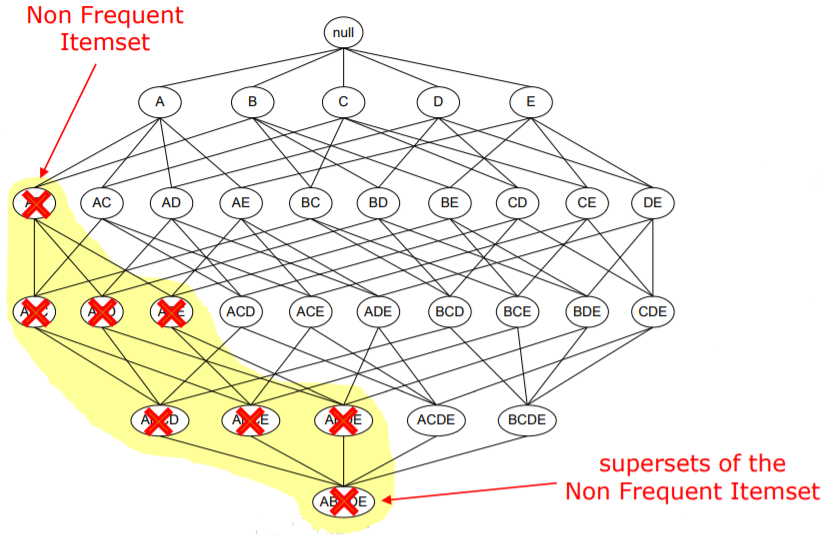
\includegraphics[height=0.5 \linewidth]{association/pict/pruning.png}
	\caption{esempio di support-based pruning}
\end{figure}

\subsubsection{Algoritmo apriori}
Genera due operazioni:
\begin{itemize}
	\item \textbf{Candidate Generation}: genera nuovi candidati k-itemset basati su (k-1)-itemset frequenti calcolati nella precedente iterazione
	\item \textbf{Candidate Pruning}: questa operazione elimina alcuni candidati k-itemset usando la strategia del support-based pruning
\end{itemize}

La complessit\`a computazionale soffre di 4 limiti:
\begin{itemize}
	\item \textit{Support threshold}: la soglia di supporto se troppo bassa non taglio molto l'albero, però non deve essere neanche troppo elevata altrimenti non considero associazioni rilevanti. 
	\item \textit{Numero di item (dimensionalit\`a)}: se il numero di item cresce, ci sar\`a bisogno di più spazio in memoria per registrare il support count degli item, inoltre bisogna considerare anche il costo dell'I/O per passare i dati.
	\item \textit{Numero di transazioni}: l'algoritmo scorre più volte tutta la lista di transazioni, pertanto un numero alto di transazioni inficia sui tempi.
	\item \textit{Avarage transaction width}: per dataset densi la lunghezza media delle transazioni tende ad essere grande. La massima lunghezza degli itemset frequenti tende ad aumentare quindi più sequenze candidato devono essere esaminate durante la generazione e support counting. In aggiunta aumenta il numero di archi traversi nell'albero durante il support counting.
\end{itemize}

\subsection{Maximal/Closed Frequent Itemsets}
\subsubsection{Rule Generation}
Ogni k-itemset frequente, Y pu\`o generare al limite $2^k-2$ regole di associazione. 

Una regola di associazione pu\`o essere estratta partizionando l'itemset Y in 2 sottoinsiemi non vuoti $\{X\}$ e $\{Y-X\}$, tale che $X \rightarrow Y -X$ soddisfa il threshold di confidenza.

\textbf{NB}: Tutte le regole generate da itemset frequenti sono esse stesse frequenti.

In pratica, il numero di itemset frequenti prodotti da transazioni possono essere molto grandi. È utile identificare itemset rappresentativi e piccoli con i quali derivare gli itemset grandi. Per questo si ragiona in due rappresentazioni:
\begin{enumerate}
	\item Maximal Frequent Itemset
	\item Closed Frequent Itemset
\end{enumerate}

\begin{defn}
	\textbf{Maximal Frequent Itemset} è definito come un Itemset Frequente per il quale nessuno dei suoi soprainsiemi immediati sono frequenti.
\end{defn}
\textbf{Maximal Frequent Itemset}: per ogni nodo si verifica il vincolo della frequenza e si definisce la frontiera dove un nodo non gode pi\`u di questa propriet\`a, corrisponde alla massima frontiera in cui mi posso spingere.

\begin{figure}[H]
	\centering
	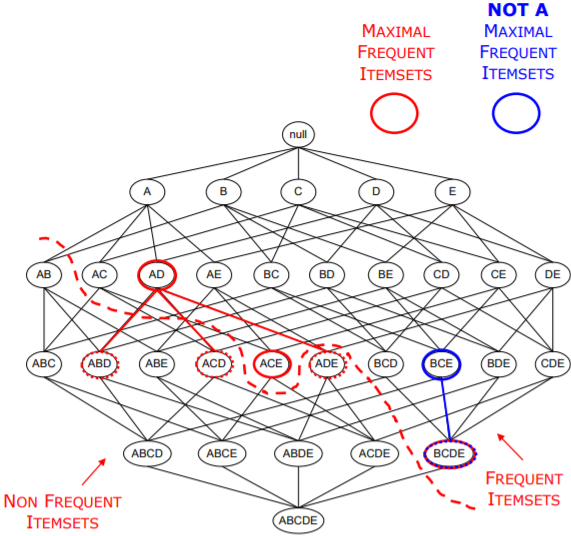
\includegraphics[height=0.7 \linewidth]{association/pict/max_freq_itemset.png}
	\caption{esempio di frontiera di maximal frequent itemset}
\end{figure}

\textbf{Nella pratica}: Un nodo \`e un Maximal Frequent Itemset se \`e frequente e se tutte le sue estensioni non sono frequenti.\\
\begin{itemize}
	\item Fornisce una rappresentazione compatta dell'insieme di itemset che cerchiamo, la pi\`u piccola espressione in cui gli itemset sono derivabili
	\item Calcolato dal più piccolo insieme di itemset dal quale tutti gli itemset frequenti possono essere derivati
	\item È praticabile solo l'algoritmo efficiente usato esplicita la ricerca dei maximal frequent itemset senza numerare tutti i suoi sottoinsiemi
\end{itemize}
Per costruzione \textit{per\`o} non ci dice quanto \`e il supporto rispetto ai suoi sottoinsiemi. In alcuni casi potrebbe servire avere una minima rappresentazione degli itemset frequenti che preservano l'informazione sul supporto.

\begin{defn}
	Un itemset X è \textbf{Closed Frequent Itemset} se nessun immediato superinsieme ha esattamente lo stesso support count di X. In ogni caso il suo supporto deve essere $\ge minsup$.
\end{defn}
Importante quando vi sono gruppi di prodotti venduti a blocco ignorando gli altri.

\textbf{Es}
\begin{figure}[H]
	\centering
	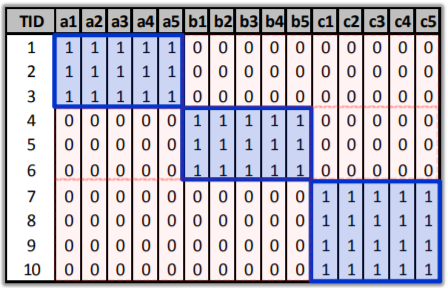
\includegraphics[height=0.5 \linewidth]{association/pict/close_freq_itemset.png}
	\caption{esempio di gruppi closed frequent itemset}
\end{figure}

Come si può notare in figura ogni gruppo di variabili (Gruppo A, B e C) è perfettamente associato e non hanno bisogno di mostrare items collegati ad altri gruppi. Assumendo che il $minsup = 20\%$, il numero totale di itemset frequenti è: $3 \cdot (2^5 -1) = 93$. In ogni caso vi sono solo 3 closed frequent itemset: 

$\{a1,a2,a3,a4,a5\}$

$\{b1,b2,b3,b4,b5\}$

$\{c1,c2,c3,c4,c5\}$


Questo tipo di itemset sono utili per rimuovere \textbf{regole di associazione ridondanti}. 
\begin{defn}
	Una regola di associazione $X \rightarrow Y$ \`e \textbf{ridondante} se esiste un'altra regola $X' \rightarrow Y'$ che rispetta certe propriet\`a. 
	\begin{itemize}
		\item $X \subseteq X'$
		\item $Y \subseteq Y'$
		\item $s(X \rightarrow Y)  = s(X' \rightarrow Y')$
		\item $c(X \rightarrow Y)  = c(X' \rightarrow Y')$
	\end{itemize}
\end{defn}

Mostriamo ora la gerarchia dei frequent itemset:
\begin{figure}[H]
	\centering
	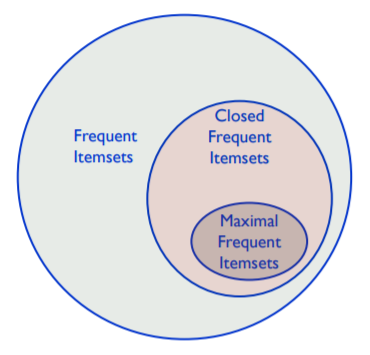
\includegraphics[height=0.45 \linewidth]{association/pict/itemset_freq.png}
	\caption{gerarchia dei frequent itemset}
\end{figure}

Come si può notare i Maximal Frequent Itemset sono inclusi nei Closed Frequent Itemset perchè nessun maxmal può avere lo stesso support count del suo immediato superset.

\subsection{Rules Evaluation (*)}
Generati gli insiemi di pattern potenzialmente utili, bisogna ordinarli in base al loro livello di attrattività per il dominio di applicazione. La valutazione della qualità viene effettuata seconodo due criteri:
\begin{itemize}
	\item \textbf{Statistical arguments}: per patterns di items indipendenti e coperti da poche transazioni. Il problema è che \textit{possono catturare relazioni spurie} nei dati, per evitare:
	\begin{itemize}
		\item \underline{Objective Interestingness Measure}: usare statistiche derivate dai dati per determinare quali pattern sono interessanti
		\item \underline{Supporto, confidenza e correlazione}
	\end{itemize}
	\item \textbf{Subjective arguments}: un pattern è considerato non interessante a meno che riveli informazioni inaspettate riguardo ai dati e alla conoscenza: \underline{es}. forte associazione tra acquisto di pannolini e birra. È difficile fare questo tipo di valutazioni, richiede una considerevole quantità di informazioni pregresse dagli esperti di domino.
\end{itemize}

Meglio cercare di applicare un approccio più \textit{oggettivo} alla valutazione: data-driven, indipendente dal dominio in cui si richiede un minimo input dagli utenti (solo dei threshold) e calcolato basandosi sulle frequenze calcolate in una \textbf{Contingency Table}.
\begin{figure}[H]
	\centering
	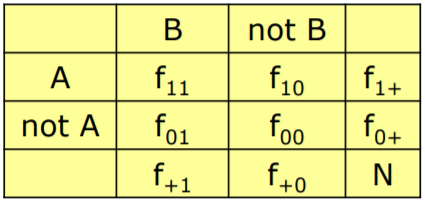
\includegraphics[height=0.2 \linewidth]{association/pict/contingency_table.png}
	\caption{contingency table}
\end{figure}
dove:
\begin{itemize}
	\item $f_{1+}$ = support count di A
	\item $f_{+1}$ = support count di B
	\item $N$ = numero di transazioni totali
\end{itemize}

Supponiamo che un direttore di un minimarket voglia analizzare la relazione tra le persone che bevono tè e persone che bevono caffè. La seguente contingency table è ottenuta considerando le transazioni disponibili:
\begin{figure}[H]
	\centering
	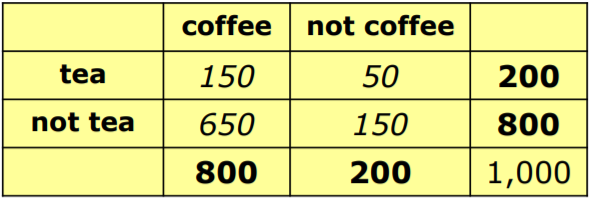
\includegraphics[height=0.2 \linewidth]{association/pict/contingency_table_es.png}
	\caption{contingency table}
\end{figure}

Ora valutiamo l'associazione: tea $\rightarrow$ coffee
\begin{itemize}
	\item $support = \frac{f_{11}}{N} = \frac{150}{1000} = 15\%$
	\item $confidence = \frac{f_{11}}{f_{1+}} = \frac{150}{200} = 75\%$
\end{itemize}

Ad una prima occhiata sembrerebbe che le persone che bevono tè tendono a bere anche caffè (vedi confidenza). Ma se notiamo le persone che bevono caffè, a prescindere dal tè sono l'$80\%$ ($\frac{800}{1000}$), mentre la frazione dei bevitori di tè che bevono caffè è solo il $75\%$.

Da questo ragionamento si può concludere che il fatto di bere tè non influisca sulle persone che bevono caffè. Infatti nonostante l`associazione abbia un alto livello di confidenza ($75\%$) non si può ignorare il supporto dell'itemset conseguente ($80\%$).

Pertanto, vengono definiti altri indici:
\begin{defn}
	\textbf{Lift}: tasso di confidenza rispetto al supporto del conseguente
	
	\[ Lift = \frac{c(A \rightarrow B)}{s(B)}\]
\end{defn}

\begin{defn}
	\textbf{Interest Factor}: equivalente al \textit{Lift} ma per attributi binari, è definito in questo modo:
	
	\[ I(A,B)  = \frac{s(A,B)}{s(A)s(B)} = \frac{Nf_{11}}{f_{1+}f_{+1}}\]
\end{defn}
I valori sono così classificati:
\begin{itemize}
	\item $=1$ se A e B sono indipendenti
	\item $>1$ se A e B sono positivamente associati
	\item $<1$ se A e B sono negativamente associati
\end{itemize}
	
\begin{defn}
	\textbf{Analisi di correlazione} (per attributi binari simmetrici): analizza la relazione tra coppie di attributi. Attributi continui possono essere analizzati con la correlazione di Pearson, la correlazione per attributi binari è misurata usando il $\phi$-coefficient:

	\[\phi = \frac{f_{11}f_{00} - f_{01}f_{10}}{\sqrt{f_{1+}f_{+1}f_{0+}f_{+0}}}\]
	
	il valore varia da $[-1,+1]$. Se gli attributi sono statisticamente indipendenti il valore è $0$.
\end{defn}

\begin{defn}
	\textbf{IS Measure} (per attributi binari asimmetrici)
	
	\[IS(A,B) = \sqrt{I(A,B)s(A,B)} = \frac{s(A,B)}{\sqrt{s(A)s(B)}}\]
	
	Il suo valore è grande quanto l'\textit{Interest Factor} e il supporto sono grandi.
	
	Se A e B sono indipendenti:
	
	\[IS(A,B) = \sqrt{s(A)s(B)}\]
	
	ha lo stesso problema della correlazione, il valore può essere grande anche per associazioni incorrelate o negativamente correlate.
\end{defn}

Vi sono altri tipi di misure per l'analisi delle relazioni tra coppie di variabili binarie.

\begin{defn} \textbf{Misure Simmetriche}

Una misura \textbf{M} è \textbf{Simmetrica} se: $M(A \rightarrow B) = M(B \rightarrow A)$

es. Interest Factor è simmetrico
\end{defn}

\begin{defn}\textbf{Misure Asimmetriche}
	
Una misura \textbf{M} è \textbf{Asimmetrica} se: $M(A \rightarrow B) \ne M(B \rightarrow A)$

es. la Confidenza è asimmetrica
\end{defn}

Di seguito gli indici più utilizzati:

\begin{table}[H]
	\centering
	\begin{tabular}{|p{5cm}|p{5cm}|}
		\hline
		Simmetrico & Asimmetrico \\
		\hline
		Correlazione ($\phi$) & Gini index \\
		Odds ratio & Mutual information \\
		Kappa & Certainty factor \\
		Interest (I) & Added value \\
		Cosine (IS) & J-measure \\
		Jaccard & Goodman-Kruskal \\
		Collective strength & \\
		\hline
	\end{tabular}
\end{table}

È importante capire che ciascuna misura è adatta per analizzare un certo tipo di associazioni come basket market analysis o document analysis. In base al caso bisogna utilizzare gli indici migliori.\\

\textbf{NB}: sono stati presentati indici relativi a valutazioni per coppie di attributi binari, ma è possibile estendere l'analisi a più di due attributi usando tabelle delle frequenti in una Contingency Table multi-dimensionale. Gli indici come il Supporto Interest Factor e IS si prestano a ciò.

\subsection{Simpson's Paradox}

Consideriamo la seguente situazione:

un direttore di un mini-market racconta di una curiosa scoperta, legata agli item birra e hot dogs. Una società di consulenza da lui pagata per analizzare i suoi dati di vendita ha scoperto che i clienti che comprano birra sono meno tentati di acquistare hot dogs rispetto a quelli che non acquistano la birra. Il direttore però è convinto del contrario, lo sa per esperienza professionale che chi acquista birra tende ad acquistare hot dogs.

Come si può risolvere il paradosso?

Consideriamo la seguente tabella:
\begin{figure}[H]
	\centering
	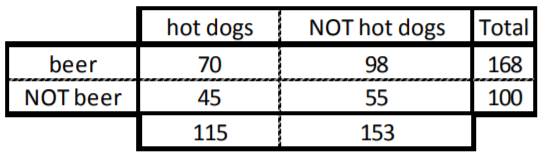
\includegraphics[height=0.2 \linewidth]{association/pict/beer_hotdog.png}
	\caption{es. birra - hot dog}
\end{figure}
Consideriamo le seguenti regole con le relative confidenze:
\begin{itemize}
	\item \{beer\} $\rightarrow$ \{hot dogs\} - confidence = $42\%$
	\item \{NOT beer\} $\rightarrow$ \{hot dogs\} - confidence = $45\%$
\end{itemize}	
Possiamo inferire che i clienti che acquistano birra sono meno inclini ($42\%$) ad acquistare hot dog rispetto a quelli che non acquistano birra ($45\%$).

Analizziamo ora gli stessi dati ma categorizzando se il cliente è single o no:
\begin{figure}[H]
	\centering
	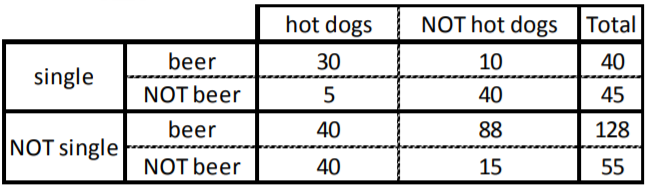
\includegraphics[height=0.2 \linewidth]{association/pict/beer_hotdog_single.png}
	\caption{es. cliente single: birra - hot dog}
\end{figure}
Pertanto posso derivare queste due coppie di regole:
\begin{itemize}
	\item Single
	\begin{itemize}
		\item \{beer\} $\rightarrow$ \{hot dogs\} - confidence = $75\%$
		\item \{NOT beer\} $\rightarrow$ \{hot dogs\} - confidence = $11\%$
	\end{itemize}
	\item NOT Single
	\begin{itemize}
		\item \{beer\} $\rightarrow$ \{hot dogs\} - confidence = $31\%$
		\item \{NOT beer\} $\rightarrow$ \{hot dogs\} - confidence = $73\%$
	\end{itemize}
\end{itemize}
Da questi dati posso affermare che: i single che acqustano birra sono più inclini ($75\%$) ad acquistare anche hot dog rispetto a quelli che non acquistano birra ($11\%$).\\

Quindi sia l'azienda di consulenza che il direttore del mini-market avevano ragione soltanto che per comprenderlo bisognava categorizzare i clienti. 

\paragraph{Paradosso di Simpson} o Yule-Simpson effect, è un paradosso della probabilità e statistica, in cui una tendenza appare in diversi gruppi di dati ma sparisce o si inverte quando questi gruppi sono combinati. \\

Bisogna applicare una appropriata stratificazione dei dati per evitare la generazione di associazioni spurie risultati dal paradosso di Simpson. 

Es. per i dati del market-basket, la catena di supermercati dovrebbe stratificarli secondo la location del negozio, mentre i dati sanitari da vari pazienti dovrebbero essere stratificati secondo fattori quali l'età o il genere.